% Created by tikzDevice version 0.12.3.1 on 2023-04-19 11:05:16
% !TEX encoding = UTF-8 Unicode
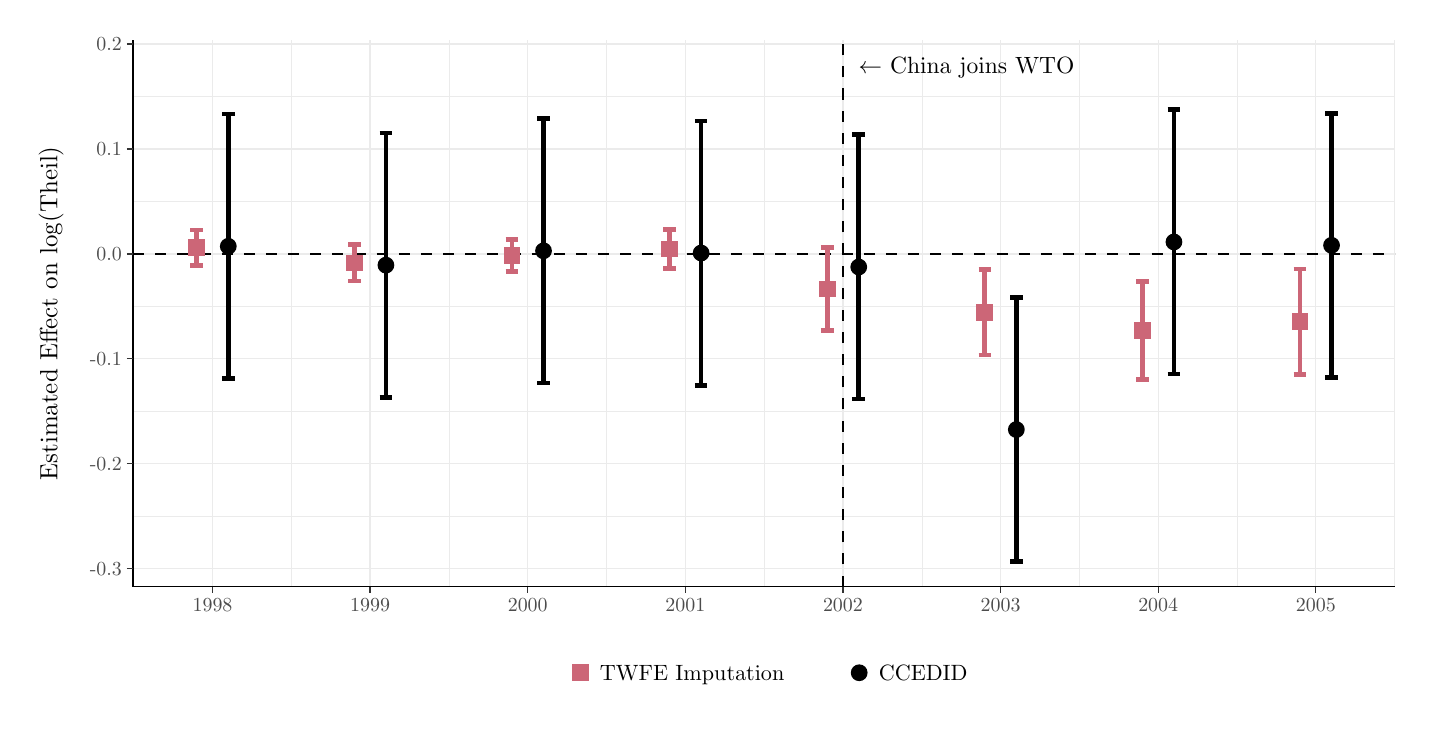
\begin{tikzpicture}[x=1pt,y=1pt]
\definecolor{fillColor}{RGB}{255,255,255}
\path[use as bounding box,fill=fillColor,fill opacity=0.00] (0,0) rectangle (498.66,249.33);
\begin{scope}
\path[clip] (  0.00,  0.00) rectangle (498.66,249.33);
\definecolor{drawColor}{RGB}{255,255,255}
\definecolor{fillColor}{RGB}{255,255,255}

\path[draw=drawColor,line width= 0.5pt,line join=round,line cap=round,fill=fillColor] ( -0.00,  0.00) rectangle (498.66,249.33);
\end{scope}
\begin{scope}
\path[clip] ( 38.10, 47.36) rectangle (494.16,244.83);
\definecolor{fillColor}{RGB}{255,255,255}

\path[fill=fillColor] ( 38.10, 47.36) rectangle (494.16,244.83);
\definecolor{drawColor}{gray}{0.92}

\path[draw=drawColor,line width= 0.2pt,line join=round] ( 38.10, 72.82) --
	(494.16, 72.82);

\path[draw=drawColor,line width= 0.2pt,line join=round] ( 38.10,110.74) --
	(494.16,110.74);

\path[draw=drawColor,line width= 0.2pt,line join=round] ( 38.10,148.65) --
	(494.16,148.65);

\path[draw=drawColor,line width= 0.2pt,line join=round] ( 38.10,186.57) --
	(494.16,186.57);

\path[draw=drawColor,line width= 0.2pt,line join=round] ( 38.10,224.48) --
	(494.16,224.48);

\path[draw=drawColor,line width= 0.2pt,line join=round] ( 38.32, 47.36) --
	( 38.32,244.83);

\path[draw=drawColor,line width= 0.2pt,line join=round] ( 95.27, 47.36) --
	( 95.27,244.83);

\path[draw=drawColor,line width= 0.2pt,line join=round] (152.23, 47.36) --
	(152.23,244.83);

\path[draw=drawColor,line width= 0.2pt,line join=round] (209.18, 47.36) --
	(209.18,244.83);

\path[draw=drawColor,line width= 0.2pt,line join=round] (266.13, 47.36) --
	(266.13,244.83);

\path[draw=drawColor,line width= 0.2pt,line join=round] (323.08, 47.36) --
	(323.08,244.83);

\path[draw=drawColor,line width= 0.2pt,line join=round] (380.03, 47.36) --
	(380.03,244.83);

\path[draw=drawColor,line width= 0.2pt,line join=round] (436.98, 47.36) --
	(436.98,244.83);

\path[draw=drawColor,line width= 0.2pt,line join=round] (493.94, 47.36) --
	(493.94,244.83);

\path[draw=drawColor,line width= 0.5pt,line join=round] ( 38.10, 53.86) --
	(494.16, 53.86);

\path[draw=drawColor,line width= 0.5pt,line join=round] ( 38.10, 91.78) --
	(494.16, 91.78);

\path[draw=drawColor,line width= 0.5pt,line join=round] ( 38.10,129.69) --
	(494.16,129.69);

\path[draw=drawColor,line width= 0.5pt,line join=round] ( 38.10,167.61) --
	(494.16,167.61);

\path[draw=drawColor,line width= 0.5pt,line join=round] ( 38.10,205.52) --
	(494.16,205.52);

\path[draw=drawColor,line width= 0.5pt,line join=round] ( 38.10,243.44) --
	(494.16,243.44);

\path[draw=drawColor,line width= 0.5pt,line join=round] ( 66.80, 47.36) --
	( 66.80,244.83);

\path[draw=drawColor,line width= 0.5pt,line join=round] (123.75, 47.36) --
	(123.75,244.83);

\path[draw=drawColor,line width= 0.5pt,line join=round] (180.70, 47.36) --
	(180.70,244.83);

\path[draw=drawColor,line width= 0.5pt,line join=round] (237.65, 47.36) --
	(237.65,244.83);

\path[draw=drawColor,line width= 0.5pt,line join=round] (294.60, 47.36) --
	(294.60,244.83);

\path[draw=drawColor,line width= 0.5pt,line join=round] (351.56, 47.36) --
	(351.56,244.83);

\path[draw=drawColor,line width= 0.5pt,line join=round] (408.51, 47.36) --
	(408.51,244.83);

\path[draw=drawColor,line width= 0.5pt,line join=round] (465.46, 47.36) --
	(465.46,244.83);
\definecolor{drawColor}{RGB}{0,0,0}

\path[draw=drawColor,line width= 0.6pt,dash pattern=on 4pt off 4pt ,line join=round] ( 38.10,167.61) -- (494.16,167.61);

\path[draw=drawColor,line width= 0.6pt,dash pattern=on 4pt off 4pt ,line join=round] (294.60, 47.36) -- (294.60,244.83);

\node[text=drawColor,anchor=base west,inner sep=0pt, outer sep=0pt, scale=  0.85] at (300.30,232.92) {$\leftarrow$ China joins WTO};
\definecolor{drawColor}{RGB}{204,102,119}

\path[draw=drawColor,line width= 1.7pt,line join=round] ( 58.83,176.27) --
	( 63.38,176.27);

\path[draw=drawColor,line width= 1.7pt,line join=round] ( 61.10,176.27) --
	( 61.10,163.31);

\path[draw=drawColor,line width= 1.7pt,line join=round] ( 58.83,163.31) --
	( 63.38,163.31);

\path[draw=drawColor,line width= 1.7pt,line join=round] (115.78,170.88) --
	(120.33,170.88);

\path[draw=drawColor,line width= 1.7pt,line join=round] (118.06,170.88) --
	(118.06,157.75);

\path[draw=drawColor,line width= 1.7pt,line join=round] (115.78,157.75) --
	(120.33,157.75);

\path[draw=drawColor,line width= 1.7pt,line join=round] (172.73,172.76) --
	(177.28,172.76);

\path[draw=drawColor,line width= 1.7pt,line join=round] (175.01,172.76) --
	(175.01,161.23);

\path[draw=drawColor,line width= 1.7pt,line join=round] (172.73,161.23) --
	(177.28,161.23);

\path[draw=drawColor,line width= 1.7pt,line join=round] (229.68,176.40) --
	(234.24,176.40);

\path[draw=drawColor,line width= 1.7pt,line join=round] (231.96,176.40) --
	(231.96,162.27);

\path[draw=drawColor,line width= 1.7pt,line join=round] (229.68,162.27) --
	(234.24,162.27);

\path[draw=drawColor,line width= 1.7pt,line join=round] (286.63,169.83) --
	(291.19,169.83);

\path[draw=drawColor,line width= 1.7pt,line join=round] (288.91,169.83) --
	(288.91,140.01);

\path[draw=drawColor,line width= 1.7pt,line join=round] (286.63,140.01) --
	(291.19,140.01);

\path[draw=drawColor,line width= 1.7pt,line join=round] (343.58,161.95) --
	(348.14,161.95);

\path[draw=drawColor,line width= 1.7pt,line join=round] (345.86,161.95) --
	(345.86,131.04);

\path[draw=drawColor,line width= 1.7pt,line join=round] (343.58,131.04) --
	(348.14,131.04);

\path[draw=drawColor,line width= 1.7pt,line join=round] (400.53,157.57) --
	(405.09,157.57);

\path[draw=drawColor,line width= 1.7pt,line join=round] (402.81,157.57) --
	(402.81,122.31);

\path[draw=drawColor,line width= 1.7pt,line join=round] (400.53,122.31) --
	(405.09,122.31);

\path[draw=drawColor,line width= 1.7pt,line join=round] (457.49,162.16) --
	(462.04,162.16);

\path[draw=drawColor,line width= 1.7pt,line join=round] (459.76,162.16) --
	(459.76,123.94);

\path[draw=drawColor,line width= 1.7pt,line join=round] (457.49,123.94) --
	(462.04,123.94);
\definecolor{drawColor}{RGB}{0,0,0}

\path[draw=drawColor,line width= 1.7pt,line join=round] ( 70.22,218.08) --
	( 74.77,218.08);

\path[draw=drawColor,line width= 1.7pt,line join=round] ( 72.49,218.08) --
	( 72.49,122.57);

\path[draw=drawColor,line width= 1.7pt,line join=round] ( 70.22,122.57) --
	( 74.77,122.57);

\path[draw=drawColor,line width= 1.7pt,line join=round] (127.17,211.28) --
	(131.72,211.28);

\path[draw=drawColor,line width= 1.7pt,line join=round] (129.45,211.28) --
	(129.45,115.77);

\path[draw=drawColor,line width= 1.7pt,line join=round] (127.17,115.77) --
	(131.72,115.77);

\path[draw=drawColor,line width= 1.7pt,line join=round] (184.12,216.46) --
	(188.68,216.46);

\path[draw=drawColor,line width= 1.7pt,line join=round] (186.40,216.46) --
	(186.40,120.95);

\path[draw=drawColor,line width= 1.7pt,line join=round] (184.12,120.95) --
	(188.68,120.95);

\path[draw=drawColor,line width= 1.7pt,line join=round] (241.07,215.65) --
	(245.63,215.65);

\path[draw=drawColor,line width= 1.7pt,line join=round] (243.35,215.65) --
	(243.35,120.14);

\path[draw=drawColor,line width= 1.7pt,line join=round] (241.07,120.14) --
	(245.63,120.14);

\path[draw=drawColor,line width= 1.7pt,line join=round] (298.02,210.61) --
	(302.58,210.61);

\path[draw=drawColor,line width= 1.7pt,line join=round] (300.30,210.61) --
	(300.30,115.10);

\path[draw=drawColor,line width= 1.7pt,line join=round] (298.02,115.10) --
	(302.58,115.10);

\path[draw=drawColor,line width= 1.7pt,line join=round] (354.97,151.85) --
	(359.53,151.85);

\path[draw=drawColor,line width= 1.7pt,line join=round] (357.25,151.85) --
	(357.25, 56.34);

\path[draw=drawColor,line width= 1.7pt,line join=round] (354.97, 56.34) --
	(359.53, 56.34);

\path[draw=drawColor,line width= 1.7pt,line join=round] (411.92,219.65) --
	(416.48,219.65);

\path[draw=drawColor,line width= 1.7pt,line join=round] (414.20,219.65) --
	(414.20,124.14);

\path[draw=drawColor,line width= 1.7pt,line join=round] (411.92,124.14) --
	(416.48,124.14);

\path[draw=drawColor,line width= 1.7pt,line join=round] (468.88,218.43) --
	(473.43,218.43);

\path[draw=drawColor,line width= 1.7pt,line join=round] (471.15,218.43) --
	(471.15,122.92);

\path[draw=drawColor,line width= 1.7pt,line join=round] (468.88,122.92) --
	(473.43,122.92);
\definecolor{fillColor}{RGB}{204,102,119}

\path[fill=fillColor] ( 58.07,166.76) --
	( 64.14,166.76) --
	( 64.14,172.82) --
	( 58.07,172.82) --
	cycle;

\path[fill=fillColor] (115.02,161.28) --
	(121.09,161.28) --
	(121.09,167.35) --
	(115.02,167.35) --
	cycle;

\path[fill=fillColor] (171.97,163.96) --
	(178.04,163.96) --
	(178.04,170.03) --
	(171.97,170.03) --
	cycle;

\path[fill=fillColor] (228.93,166.30) --
	(234.99,166.30) --
	(234.99,172.37) --
	(228.93,172.37) --
	cycle;

\path[fill=fillColor] (285.88,151.89) --
	(291.94,151.89) --
	(291.94,157.95) --
	(285.88,157.95) --
	cycle;

\path[fill=fillColor] (342.83,143.46) --
	(348.89,143.46) --
	(348.89,149.53) --
	(342.83,149.53) --
	cycle;

\path[fill=fillColor] (399.78,136.91) --
	(405.85,136.91) --
	(405.85,142.98) --
	(399.78,142.98) --
	cycle;

\path[fill=fillColor] (456.73,140.02) --
	(462.80,140.02) --
	(462.80,146.09) --
	(456.73,146.09) --
	cycle;
\definecolor{fillColor}{RGB}{0,0,0}

\path[fill=fillColor] ( 72.49,170.32) circle (  3.03);

\path[fill=fillColor] (129.45,163.52) circle (  3.03);

\path[fill=fillColor] (186.40,168.70) circle (  3.03);

\path[fill=fillColor] (243.35,167.90) circle (  3.03);

\path[fill=fillColor] (300.30,162.85) circle (  3.03);

\path[fill=fillColor] (357.25,104.10) circle (  3.03);

\path[fill=fillColor] (414.20,171.90) circle (  3.03);

\path[fill=fillColor] (471.15,170.68) circle (  3.03);
\end{scope}
\begin{scope}
\path[clip] (  0.00,  0.00) rectangle (498.66,249.33);
\definecolor{drawColor}{RGB}{0,0,0}

\path[draw=drawColor,line width= 0.5pt,line join=round] ( 38.10, 47.36) --
	( 38.10,244.83);
\end{scope}
\begin{scope}
\path[clip] (  0.00,  0.00) rectangle (498.66,249.33);
\definecolor{drawColor}{gray}{0.30}

\node[text=drawColor,anchor=base east,inner sep=0pt, outer sep=0pt, scale=  0.72] at ( 34.05, 51.38) {-0.3};

\node[text=drawColor,anchor=base east,inner sep=0pt, outer sep=0pt, scale=  0.72] at ( 34.05, 89.30) {-0.2};

\node[text=drawColor,anchor=base east,inner sep=0pt, outer sep=0pt, scale=  0.72] at ( 34.05,127.21) {-0.1};

\node[text=drawColor,anchor=base east,inner sep=0pt, outer sep=0pt, scale=  0.72] at ( 34.05,165.13) {0.0};

\node[text=drawColor,anchor=base east,inner sep=0pt, outer sep=0pt, scale=  0.72] at ( 34.05,203.04) {0.1};

\node[text=drawColor,anchor=base east,inner sep=0pt, outer sep=0pt, scale=  0.72] at ( 34.05,240.96) {0.2};
\end{scope}
\begin{scope}
\path[clip] (  0.00,  0.00) rectangle (498.66,249.33);
\definecolor{drawColor}{gray}{0.20}

\path[draw=drawColor,line width= 0.5pt,line join=round] ( 35.85, 53.86) --
	( 38.10, 53.86);

\path[draw=drawColor,line width= 0.5pt,line join=round] ( 35.85, 91.78) --
	( 38.10, 91.78);

\path[draw=drawColor,line width= 0.5pt,line join=round] ( 35.85,129.69) --
	( 38.10,129.69);

\path[draw=drawColor,line width= 0.5pt,line join=round] ( 35.85,167.61) --
	( 38.10,167.61);

\path[draw=drawColor,line width= 0.5pt,line join=round] ( 35.85,205.52) --
	( 38.10,205.52);

\path[draw=drawColor,line width= 0.5pt,line join=round] ( 35.85,243.44) --
	( 38.10,243.44);
\end{scope}
\begin{scope}
\path[clip] (  0.00,  0.00) rectangle (498.66,249.33);
\definecolor{drawColor}{RGB}{0,0,0}

\path[draw=drawColor,line width= 0.5pt,line join=round] ( 38.10, 47.36) --
	(494.16, 47.36);
\end{scope}
\begin{scope}
\path[clip] (  0.00,  0.00) rectangle (498.66,249.33);
\definecolor{drawColor}{gray}{0.20}

\path[draw=drawColor,line width= 0.5pt,line join=round] ( 66.80, 45.11) --
	( 66.80, 47.36);

\path[draw=drawColor,line width= 0.5pt,line join=round] (123.75, 45.11) --
	(123.75, 47.36);

\path[draw=drawColor,line width= 0.5pt,line join=round] (180.70, 45.11) --
	(180.70, 47.36);

\path[draw=drawColor,line width= 0.5pt,line join=round] (237.65, 45.11) --
	(237.65, 47.36);

\path[draw=drawColor,line width= 0.5pt,line join=round] (294.60, 45.11) --
	(294.60, 47.36);

\path[draw=drawColor,line width= 0.5pt,line join=round] (351.56, 45.11) --
	(351.56, 47.36);

\path[draw=drawColor,line width= 0.5pt,line join=round] (408.51, 45.11) --
	(408.51, 47.36);

\path[draw=drawColor,line width= 0.5pt,line join=round] (465.46, 45.11) --
	(465.46, 47.36);
\end{scope}
\begin{scope}
\path[clip] (  0.00,  0.00) rectangle (498.66,249.33);
\definecolor{drawColor}{gray}{0.30}

\node[text=drawColor,anchor=base,inner sep=0pt, outer sep=0pt, scale=  0.72] at ( 66.80, 38.35) {1998};

\node[text=drawColor,anchor=base,inner sep=0pt, outer sep=0pt, scale=  0.72] at (123.75, 38.35) {1999};

\node[text=drawColor,anchor=base,inner sep=0pt, outer sep=0pt, scale=  0.72] at (180.70, 38.35) {2000};

\node[text=drawColor,anchor=base,inner sep=0pt, outer sep=0pt, scale=  0.72] at (237.65, 38.35) {2001};

\node[text=drawColor,anchor=base,inner sep=0pt, outer sep=0pt, scale=  0.72] at (294.60, 38.35) {2002};

\node[text=drawColor,anchor=base,inner sep=0pt, outer sep=0pt, scale=  0.72] at (351.56, 38.35) {2003};

\node[text=drawColor,anchor=base,inner sep=0pt, outer sep=0pt, scale=  0.72] at (408.51, 38.35) {2004};

\node[text=drawColor,anchor=base,inner sep=0pt, outer sep=0pt, scale=  0.72] at (465.46, 38.35) {2005};
\end{scope}
\begin{scope}
\path[clip] (  0.00,  0.00) rectangle (498.66,249.33);
\definecolor{drawColor}{RGB}{0,0,0}

\node[text=drawColor,rotate= 90.00,anchor=base,inner sep=0pt, outer sep=0pt, scale=  0.90] at ( 10.70,146.10) {Estimated Effect on $\log($Theil$)$};
\end{scope}
\begin{scope}
\path[clip] (  0.00,  0.00) rectangle (498.66,249.33);
\definecolor{fillColor}{RGB}{255,255,255}

\path[fill=fillColor] (178.11,  4.50) rectangle (354.15, 27.95);
\end{scope}
\begin{scope}
\path[clip] (  0.00,  0.00) rectangle (498.66,249.33);
\definecolor{fillColor}{RGB}{255,255,255}

\path[fill=fillColor] (185.45,  9.00) rectangle (213.91, 23.45);
\end{scope}
\begin{scope}
\path[clip] (  0.00,  0.00) rectangle (498.66,249.33);
\definecolor{fillColor}{RGB}{204,102,119}

\path[fill=fillColor] (196.65, 13.19) --
	(202.71, 13.19) --
	(202.71, 19.26) --
	(196.65, 19.26) --
	cycle;
\end{scope}
\begin{scope}
\path[clip] (  0.00,  0.00) rectangle (498.66,249.33);
\definecolor{fillColor}{RGB}{255,255,255}

\path[fill=fillColor] (286.25,  9.00) rectangle (314.70, 23.45);
\end{scope}
\begin{scope}
\path[clip] (  0.00,  0.00) rectangle (498.66,249.33);
\definecolor{fillColor}{RGB}{0,0,0}

\path[fill=fillColor] (300.47, 16.23) circle (  3.03);
\end{scope}
\begin{scope}
\path[clip] (  0.00,  0.00) rectangle (498.66,249.33);
\definecolor{drawColor}{RGB}{0,0,0}

\node[text=drawColor,anchor=base west,inner sep=0pt, outer sep=0pt, scale=  0.80] at (206.75, 13.47) {TWFE Imputation};
\end{scope}
\begin{scope}
\path[clip] (  0.00,  0.00) rectangle (498.66,249.33);
\definecolor{drawColor}{RGB}{0,0,0}

\node[text=drawColor,anchor=base west,inner sep=0pt, outer sep=0pt, scale=  0.80] at (307.55, 13.47) {CCEDID};
\end{scope}
\end{tikzpicture}
